\documentclass[tikz,border=8pt]{standalone}
% Shared look for every TikZ diagram. Load with % Shared look for every TikZ diagram. Load with % Shared look for every TikZ diagram. Load with \input{../../tools/tikz-style.tex}
\usepackage[T1]{fontenc}
\usepackage{lmodern}
\renewcommand{\sfdefault}{lmr}  % diagrams use the same serif as the text
\usetikzlibrary{arrows.meta, positioning, shapes.geometric, calc, fit, backgrounds}
\definecolor{cblue}{HTML}{4C78A8}
\definecolor{corange}{HTML}{F58518}
\definecolor{cgreen}{HTML}{54A24B}
\definecolor{cred}{HTML}{E45756}
\definecolor{cpurple}{HTML}{B279A2}
\definecolor{cgrey}{HTML}{6B6B6B}
\tikzset{
  every picture/.style={font=\sffamily, line width=1.2pt},
  box/.style={draw=#1, fill=#1!12, rounded corners=4pt, align=center, inner sep=7pt, minimum height=1.1cm},
  box/.default=cgrey,
  arrow/.style={-{Stealth[length=3mm]}, draw=cgrey, line width=1.4pt},
  title/.style={font=\sffamily\bfseries\Large},
  note/.style={font=\sffamily\small, text=cgrey, align=center},
}
\AtBeginDocument{\hyphenpenalty=10000 \exhyphenpenalty=10000}

\usepackage[T1]{fontenc}
\usepackage{lmodern}
\renewcommand{\sfdefault}{lmr}  % diagrams use the same serif as the text
\usetikzlibrary{arrows.meta, positioning, shapes.geometric, calc, fit, backgrounds}
\definecolor{cblue}{HTML}{4C78A8}
\definecolor{corange}{HTML}{F58518}
\definecolor{cgreen}{HTML}{54A24B}
\definecolor{cred}{HTML}{E45756}
\definecolor{cpurple}{HTML}{B279A2}
\definecolor{cgrey}{HTML}{6B6B6B}
\tikzset{
  every picture/.style={font=\sffamily, line width=1.2pt},
  box/.style={draw=#1, fill=#1!12, rounded corners=4pt, align=center, inner sep=7pt, minimum height=1.1cm},
  box/.default=cgrey,
  arrow/.style={-{Stealth[length=3mm]}, draw=cgrey, line width=1.4pt},
  title/.style={font=\sffamily\bfseries\Large},
  note/.style={font=\sffamily\small, text=cgrey, align=center},
}
\AtBeginDocument{\hyphenpenalty=10000 \exhyphenpenalty=10000}

\usepackage[T1]{fontenc}
\usepackage{lmodern}
\renewcommand{\sfdefault}{lmr}  % diagrams use the same serif as the text
\usetikzlibrary{arrows.meta, positioning, shapes.geometric, calc, fit, backgrounds}
\definecolor{cblue}{HTML}{4C78A8}
\definecolor{corange}{HTML}{F58518}
\definecolor{cgreen}{HTML}{54A24B}
\definecolor{cred}{HTML}{E45756}
\definecolor{cpurple}{HTML}{B279A2}
\definecolor{cgrey}{HTML}{6B6B6B}
\tikzset{
  every picture/.style={font=\sffamily, line width=1.2pt},
  box/.style={draw=#1, fill=#1!12, rounded corners=4pt, align=center, inner sep=7pt, minimum height=1.1cm},
  box/.default=cgrey,
  arrow/.style={-{Stealth[length=3mm]}, draw=cgrey, line width=1.4pt},
  title/.style={font=\sffamily\bfseries\Large},
  note/.style={font=\sffamily\small, text=cgrey, align=center},
}
\AtBeginDocument{\hyphenpenalty=10000 \exhyphenpenalty=10000}

\begin{document}
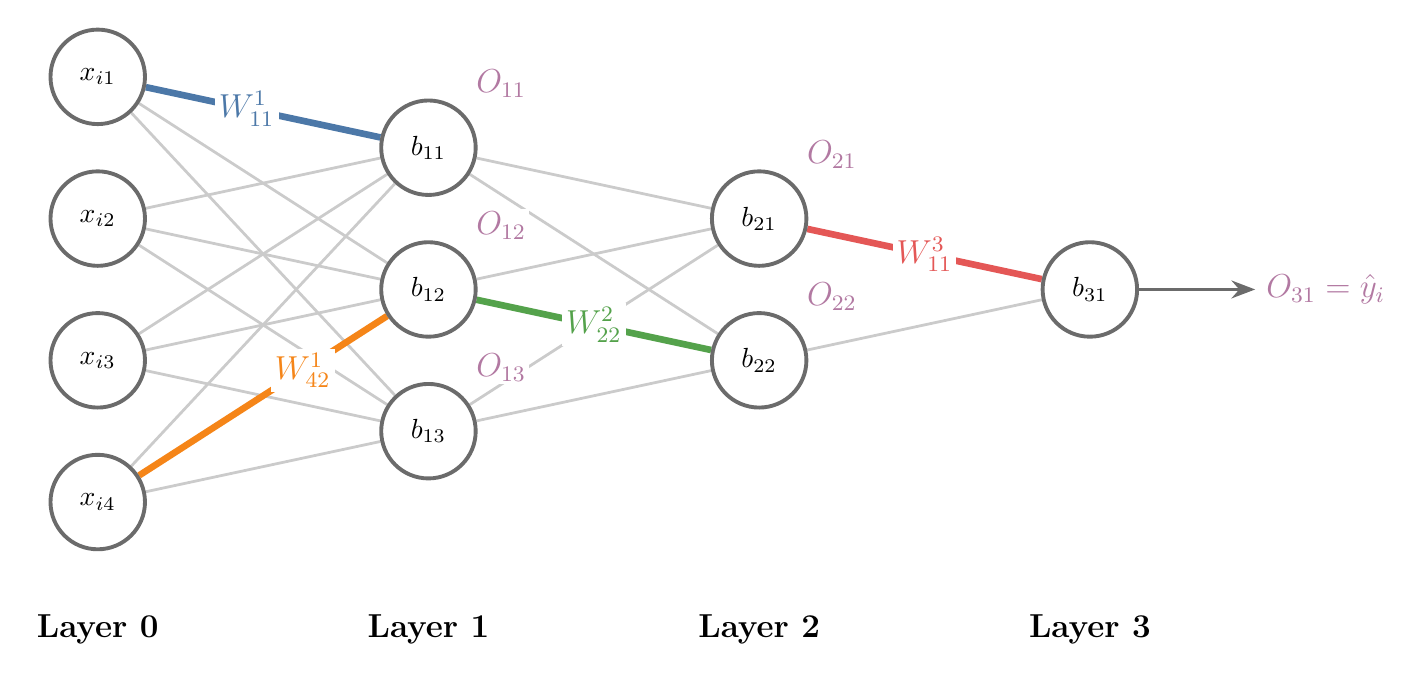
\begin{tikzpicture}[x=4.2cm, y=1.8cm,
  neuron/.style={circle, draw=cgrey, fill=white, minimum size=1.2cm, line width=1.4pt, font=\sffamily\normalsize},
  lab/.style={fill=white, inner sep=1.5pt, font=\sffamily\large}]
  \foreach \i in {1,...,4} \node[neuron] (a\i) at (0, 2.5-\i) {$x_{i\i}$};
  \foreach \j in {1,2,3} \node[neuron] (b\j) at (1, 2-\j) {$b_{1\j}$};
  \foreach \j in {1,2} \node[neuron] (c\j) at (2, 1.5-\j) {$b_{2\j}$};
  \node[neuron] (d1) at (3, 0) {$b_{31}$};
  \begin{scope}[on background layer]
  \foreach \i in {1,...,4} \foreach \j in {1,2,3} \draw[cgrey!35, line width=1pt] (a\i) -- (b\j);
  \foreach \i in {1,2,3} \foreach \j in {1,2} \draw[cgrey!35, line width=1pt] (b\i) -- (c\j);
  \foreach \i in {1,2} \draw[cgrey!35, line width=1pt] (c\i) -- (d1);
  % highlighted weights
  \draw[cblue, line width=2.4pt] (a1) -- (b1);
  \draw[corange, line width=2.4pt] (a4) -- (b2);
  \draw[cgreen, line width=2.4pt] (b2) -- (c2);
  \draw[cred, line width=2.4pt] (c1) -- (d1);
  \end{scope}
  \node[lab, text=cblue] at ($(a1)!0.45!(b1)$) {$W^{1}_{11}$};
  \node[lab, text=corange] at ($(a4)!0.62!(b2)$) {$W^{1}_{42}$};
  \node[lab, text=cgreen] at ($(b2)!0.5!(c2)$) {$W^{2}_{22}$};
  \node[lab, text=cred] at ($(c1)!0.5!(d1)$) {$W^{3}_{11}$};
  % outputs
  \foreach \n/\t in {b1/O_{11}, b2/O_{12}, b3/O_{13}, c1/O_{21}, c2/O_{22}}
    \node[font=\sffamily\large, text=cpurple, fill=white, inner sep=1pt] at ($(\n)+(0.22,0.45)$) {$\t$};
  \draw[arrow] (d1) -- ++(0.5,0) node[right, text=cpurple, font=\sffamily\large] {$O_{31} = \hat{y}_i$};
  \foreach \x/\t in {0/Layer 0, 1/Layer 1, 2/Layer 2, 3/Layer 3}
    \node[font=\sffamily\large\bfseries] at (\x, -2.4) {\t};
\end{tikzpicture}
\end{document}
